% --- tv3_quocviet.tex ---
% Phân tích Nhóm 3: Phân tích Khách hàng

\noindent\textbf{3. Kết quả phân tích \& Trực quan hóa:}

\begin{figure}[H]
    \centering
    
\includegraphics[width=0.9\textwidth]{images/customer_analysis/cust_spend_age_gender.png}
    \caption{Tổng chi tiêu theo nhóm tuổi và giới tính}
    \label{fig:cust_spend_age_gender}
\end{figure}

\textbf{a. Phân bổ khách hàng theo độ tuổi và giới tính --- Nhóm nào chi tiêu nhiều nhất?}
\\
Biểu đồ \ref{fig:cust_spend_age_gender} sử dụng Grouped Bar Chart với trục X là nhóm tuổi (18--24, 25--34, 35--44, 45--54, 55--69), chiều cao cột biểu thị tổng chi tiêu khả dụng (nghìn USD, đã loại trừ đơn hàng hoàn trả) và màu sắc phân biệt giới tính. Kết quả cho thấy \textbf{nhóm 55--69 tuổi chi tiêu cao nhất} với mức \$748K (Female) và \$718K (Male), phản ánh sức mua vượt trội của nhóm khách hàng đã tích lũy thu nhập ổn định. Ngược lại, nhóm \textbf{18--24 tuổi} có chi tiêu thấp nhất toàn sàn (Female: \$376K, Male: \$361K) do thu nhập hạn chế hoặc mới tham gia thị trường lao động. Đáng chú ý, chi tiêu tăng đều theo độ tuổi ở cả hai giới chính mà không có dấu hiệu bão hòa --- đây là tín hiệu tích cực cho chiến lược nhắm đến nhóm khách hàng trung niên và lớn tuổi. Ngoài ra, \textbf{Female} có xu hướng chi tiêu cao hơn Male ở nhóm 45--69, trong khi Male chiếm ưu thế nhẹ ở nhóm 25--44, cho thấy sự khác biệt hành vi mua sắm theo vòng đời rõ rệt.

\begin{figure}[H]
    \centering
    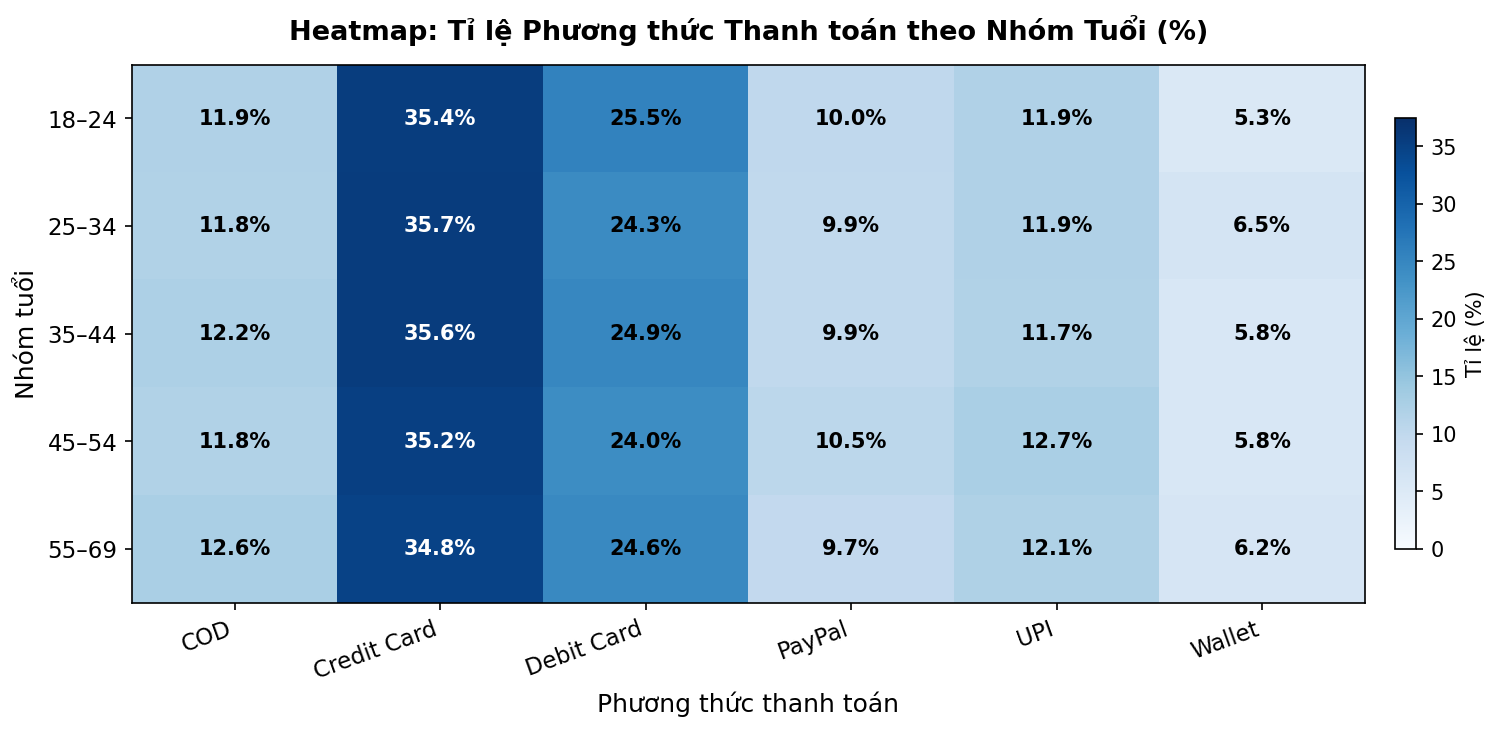
\includegraphics[width=0.9\textwidth]{images/customer_analysis/cust_payment_heatmap.png}
    \caption{Heatmap tỉ lệ phương thức thanh toán theo nhóm tuổi (\%)}
    \label{fig:cust_payment_heatmap}
\end{figure}

\textbf{b. Phương thức thanh toán nào được ưa chuộng nhất? --- Có sự khác biệt theo nhóm tuổi không?}
\\
Biểu đồ \ref{fig:cust_payment_heatmap} trình bày dưới dạng Heatmap với các ô màu xanh (độ đậm tỉ lệ thuận với phần trăm sử dụng) và giá trị \% được ghi trực tiếp trên từng ô. \textbf{Credit Card} là phương thức thống trị ở \textit{tất cả} các nhóm tuổi với tỉ lệ dao động \textbf{35--36\%}, phản ánh sự tin tưởng vào bảo mật thẻ và các ưu đãi hoàn tiền đi kèm. \textbf{Debit Card} xếp thứ hai với khoảng \textbf{24--25\%} và khá đồng đều qua mọi độ tuổi, cho thấy đây là lựa chọn phổ quát không phụ thuộc vào thế hệ. Điểm đáng lưu ý là \textbf{COD (thanh toán khi nhận hàng)} duy trì ổn định ở mức \textbf{$\sim$12\%} và không giảm mạnh ở nhóm cao tuổi như kỳ vọng, điều này cho thấy tâm lý an toàn khi mua sắm trực tuyến vẫn còn phổ biến. \textbf{UPI} và \textbf{PayPal} lần lượt chiếm khoảng \textbf{12\%} và \textbf{10\%} đồng đều qua mọi nhóm --- gợi ý cả hai đã được phổ cập rộng rãi bất kể tuổi tác. \textbf{Wallet} có tỉ lệ thấp nhất ($\sim$6\%) và không có sự chênh lệch rõ rệt theo tuổi, điều này mâu thuẫn với kỳ vọng giới trẻ dùng ví nhiều hơn, có thể do ưu đãi Credit Card hấp dẫn hơn tạo ra hiệu ứng thay thế.

\begin{figure}[H]
    \centering
    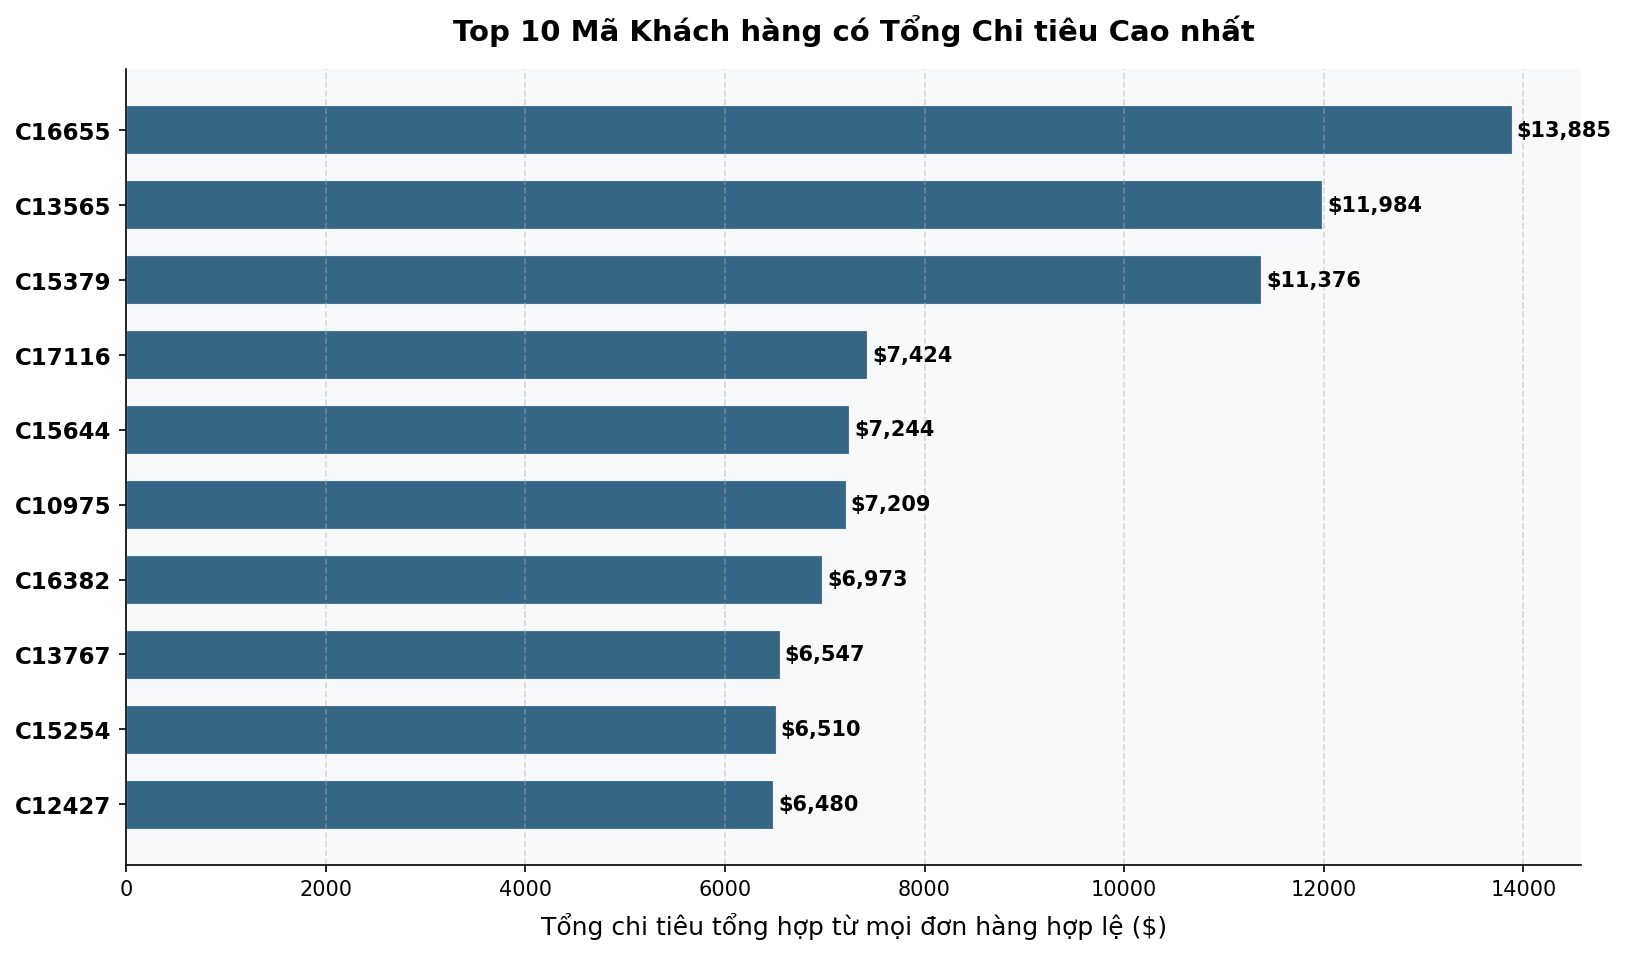
\includegraphics[width=0.9\textwidth]{images/customer_analysis/cust_top10.png}
    \caption{Top 10 khách hàng theo tổng chi tiêu tích lũy (USD)}
    \label{fig:cust_top10}
\end{figure}

\textbf{c. Top khách hàng có giá trị cao nhất (theo tổng chi tiêu) là ai?}
\\
Biểu đồ \ref{fig:cust_top10} sử dụng Horizontal Bar Chart hiển thị, sắp xếp theo tổng chi tiêu thực tế (đã loại trừ đơn hàng hoàn trả) tổng hợp trực tiếp từ mã \texttt{customer\_id}. Khách hàng \textbf{C16655} dẫn đầu cực kỳ ấn tượng với tổng chi tiêu \textbf{\$13,885} --- vượt qua đáng kể so với nhóm bám đuổi, phản ánh mức độ tập trung giá trị cao ở một số ít VIP customer. Việc định danh và phân loại nhóm tinh hoa này sẽ dựa hoàn toàn trên mã \texttt{customer\_id} do biến động về thông tin định dạng cá nhân. Đáng chú ý, toàn bộ 10 định danh xếp đầu bảng này đều đã vượt qua các mốc chi tiêu rất lớn trên sàn, trong đó ngưỡng \textbf{\$6,480} của tài khoản lọt vào top 10 là mốc tham chiếu quan trọng để nền tảng tự động thiết lập chính sách đãi ngộ, trao tặng voucher lớn trong các chương trình khách hàng thân thiết (loyalty programs) sắp tới.

\vspace{0.3cm}
\noindent\textbf{4. Đưa ra quyết định trong tương lai:}
\begin{itemize}
    \item \textbf{Cá nhân hóa marketing cho nhóm VIP:} Xây dựng kịch bản chăm sóc riêng cho thực thể dẫn đầu như khách hàng \textbf{C16655} và nhóm Top 10 để duy trì sự trung thành.
    \item \textbf{Kích cầu nhóm khách hàng trung niên (45--69):} Thiết kế các chiến dịch quảng cáo nhắm mục tiêu vào nhóm tuổi này vì họ có sức mua lớn nhất, đặc biệt là nữ giới trong nhóm 55--69 tuổi.
    \item \textbf{Hợp tác đẩy mạnh thanh toán thẻ:} Liên kết với các ngân hàng để tung ra thêm ưu đãi hoàn tiền (cashback) cho \textbf{Credit Card} vì đây là phương thức chủ đạo được mọi nhóm tuổi tin dùng. Đồng thời, cần cải thiện trải nghiệm \textbf{Wallet} để thu hút thêm đối tượng trẻ tuổi.
\end{itemize}

